

\section{Implementation}
\label{sec:implementation}
\begin{wraptable}[11]{r}{0.32\textwidth}
	\vspace{-1.5em} 
	\centering
	\begin{tabular}{@{} l S[table-format=5.0] @{}}
		\toprule
		\textbf{Module}                & {\textbf{LoC}} \\
		\midrule
		Input \& Parsing               &  1723          \\
		Model Construction             &  5561          \\
		Petri--Net Conversion           &   843          \\
		Reachability          &  2628          \\
		Proof Checking                 &  3240          \\
		Utilities                      &  2160          \\
		Testing \& Evaluation          &  2118          \\
		\midrule
		\textbf{Total}                 & \textbf{18273} \\
		\bottomrule
	\end{tabular}
	\caption{Lines of Code}
	\label{tab:loc_summary2}
\end{wraptable}
%\vspace{-1.5\baselineskip} % nudge following text up a bit
We implemented our approach in \toolname{}~\cite{ArtifactRepository}, a publicly available toolchain consisting of over $18{,}200$ LoC written mostly in \texttt{Rust} (see Table~\ref{tab:loc_summary2}).
%
%We next elaborate on the architecture of our tool and the various optimizations we added to allow it to run efficiently.
%
%For the underlying Petri Net model checker, we use SMPT~\cite{AmDa23} which supports \textit{unbounded} reachability queries (see Appendix~\ref{appendix:smpt}).
%, and which uses Z3 as an underlying SMT solver~\cite{DeBj08}. 
%and which we extended to support our setting (for example, we needed to extend the solver to support proof generation). 
%
%We note that other off-the-shelf solvers can be used as well.

%The implementation..

%\begin{enumerate}
%	\item The extra things we did to make the thing actually run
%	\item Code architecture
%	\item Optimizations
%\end{enumerate}

%\newpage
\subsection{Code Architecture}

%\begin{tabular}{|l|r|}
%	\hline
%	\textbf{Module} & \textbf{LoC} \\
%	\hline
%	Input \& Parsing                             & 1723  \\
%	\hline
%	Model Construction                           & 5561  \\
%	\hline
%	Petri-Net Conversion                         & 843   \\
%	\hline
%	Reachability Checking                        & 2628  \\
%	\hline
%	Proof Checking                               & 3240  \\
%	\hline
%	Utilities                                       & 2160  \\
%	\hline
%	Testing \& Evaluation               & 2118  \\
%	\hline
%	\textbf{Total}                               & \textbf{18273} \\
%	\hline
%\end{tabular}


%
%\begin{table}[ht]
%	\centering
%	\label{tab:loc_summary}
%	\begin{tabular}{@{} l S[table-format=5.0] @{}}
%		\toprule
%		\textbf{Module}                & {\textbf{LoC}} \\
%		\midrule
%		Input \& Parsing               &  1723          \\
%		Model Construction             &  5561          \\
%		Petri–Net Conversion           &   843          \\
%		Reachability Checking          &  2628          \\
%		Proof Checking                 &  3240          \\
%		Utilities                      &  2160          \\
%		Testing \& Evaluation          &  2118          \\
%		\midrule
%		\textbf{Total}                 & \textbf{18273}          \\
%		\bottomrule
%	\end{tabular}
%	\caption{Lines of Code by Module}
%\end{table}
%

% Then, where you want the table wrapped to the right:
%
% this table summarizes the values without whitespaces/comments and without the code for SMPT (or the wrapper) or the carfo and toml files
%
%\begin{wraptable}[8]{r}{0.32\textwidth}
%	\centering
%	\begin{tabular}{@{} l S[table-format=5.0] @{}}
%		\toprule
%		\textbf{Module}                & {\textbf{LoC}} \\
%		\midrule
%		Input \& Parsing               &  1723          \\
%		Model Construction             &  5561          \\
%		Petri–Net Conversion           &   843          \\
%		Reachability          &  2628          \\
%		Proof Checking                 &  3240          \\
%		Utilities                      &  2160          \\
%		Testing \& Evaluation          &  2118          \\
%		\midrule
%		\textbf{Total}                 & \textbf{18273} \\
%		\bottomrule
%	\end{tabular}
%	\caption{Lines of Code (LoC)}
%	\label{tab:loc_summary2}
%\end{wraptable}
%
%\noindent
%
\toolname{} implements an end-to-end serializability checker for a given input program. If the program is serializable, we return a proof thereof; otherwise, if it is not serializable, a counterexample is given to the user for an interleaving that can result in request/response pairs that are unattainable in any serial execution.
%
Our workflow translates the decidability problem to an equivalent Petri net reachability question (for an unbounded number of tokens), in which (i) the Petri net represents all possible interleavings of the program; and (ii) the reachability query represents a semilinear set (equivalently, a Presburger arithmetic encoding) of all request/response pairs that \textit{cannot} be obtained by any serial execution.
%
As Petri net reachability is \texttt{Ackermann}-complete~\cite{CzWo22}, we added various optimizations to expedite the search process, both at the PN level and the property-encoding level.
%
The pipeline of \toolname{} is depicted in Fig.~\ref{fig:full_program_flow}, and includes:
 

\begin{enumerate}
	\item \textbf{Input \& parsing.} 
	Our framework receives either a \texttt{SER} program with the syntax described in~\Cref{sec:problem-definition}; or a \texttt{JSON} file directly encoding a network system. In the case of the former, an additional step takes place, parsing the input %(using the \texttt{parser.rs} module) 
	to an expression tree that is translated to the equivalent NS.
%	, represented as a struct in the \texttt{ns.rs} module. 
	
	\item \textbf{Petri net conversion.} The NS is then translated into a Petri net 
%	(see the \texttt{petri.rs} module) 
which represents all possible interleavings. 
%	.as depicted, for example, in subsec.~\ref{subsec:ns-not-serializable}.
%	Each place represents a state (either global or local) or a response. Each token represents a single in-flight request or a terminated response. 
The PN is encoded in the de facto standard \texttt{NET} format, to support off-the-shelf PN model checkers. 
	
	\item \textbf{Semilinear conversion.} 
%	This includes a set of modules (\texttt{kleene.rs}, \texttt{semilinear.rs}, and \texttt{presburger.rs}) which 
We generate a semilinear set encoding all non-serializable outputs, via translation of the serialized NFA (e.g., Fig.~\ref{fig:code2ExampleNFA}) to a regex, which is then projected (via the Parikh image) and complemented. 
%	This conversion is done by the following pipeline: (1) the NS is translated to an NFA encoding all possible request/response pairs of the input program; (2) This NFA is translated to a regex (via Kleene's Theorem) and then projected (via the Parikh Image) to a semilinear set. The (finite) encoding of the semilinear set symbolically represents all outputs attained via serializable executions of the program, running for an unbounded number of steps; (3) finally, we complement the semilinear set to encode all outputs unattainable via serial executions. 
	At the end of the pipeline, an \texttt{XML}-formatted output encodes a reachability query that encapsulates constraints over the PN token count.
	
	
	\item \textbf{Reachability engine.} The PN and the reachability query are fed to a  PN model checker, which combines \textit{bounded model checking} (BMC)~\cite{BiCiClZh99} in search of a counterexample; and \textit{state equation reasoning}~\cite{Mu77} in order to prove non-reachability. 
%	This engine is implemented in the \texttt{reachability.rs} and \texttt{reachability\_with\_proofs.rs}  modules.
	%
	In order to expedite the search, ``large'' (PN, query) pairs are replaced with multiple sliced PNs (generated by the reachability engine), each coupled with a sub-query encoding a separate disjunct. 
%	of the original query.
%	We iteratively solve the 
The disjuncts are solved on the fly, until reaching \texttt{SAT}, in which case, we have a counterexample; otherwise, if all disjuncts are \texttt{UNSAT}, we render the original program as serializable.
	
	
	\item \textbf{Proof \& certification.} 
	If \texttt{SAT}, we reconstruct and validate an NS-level counterexample. Otherwise, if all disjuncts are \texttt{UNSAT}, we extract per-disjunct proofs and ``stitch'' these to a single inductive serializability certificate, which we then project to the NS and validate (i) initiation, (ii) inductiveness, and (iii) query refutation.
	%
%	If the query is \texttt{SAT}, we reconstruct a non-serializable NS-level execution and validate its correctness. Otherwise, if all disjuncts are \texttt{UNSAT}, our proof module extracts a separate proof for each disjunct. We subsequently ``stitch'' these proofs to a single inductive invariant, and project it to the NS-level, representing a full inductive proof certificate for serializability. Our checker also validates that the inductive invariant is correct, i.e., (i) includes the initial state; (ii) is inductive with regard to the transitions; and (iii) implies that the reachability query is \texttt{UNSAT}.
	%, and hence, implying serializability. 
	
	
	\item \textbf{Instrumentation \& logging.} Throughout the pipeline, we record various intermediate representations and performance metrics.  
%	input size and performance metrics (number of places, transitions, constraint complexity, timings) 
%
%The logger outputs 
%We generate \texttt{CSV} and \texttt{JSON} logs along with
% analysis. 
	%
%	We also assemble 
%an \texttt{HTML} report embedding the original net, symbolic constraints, reachability results, proofs, etc.
%	\item \textbf{Debug Report Generation.} Finally, a human-readable \texttt{HTML} report is assembled: it embeds the original net, symbolic constraints, reachability results, proof outlines, and profiling graphs. This interactive report allows users to drill down into each transition firing, constraint check, and proof obligation.
	
%	\item \textbf{Output Delivery.} The crate exposes a simple CLI and library API. Users obtain either a Boolean reachability verdict (with optional certificate), raw log files, or a full HTML debug report, depending on invocation flags.
	
%	\item \textbf{Optimizations.} As formalized in the previous section, we implement multiple optimizations throughout the process.
%	, both for representing the semilinear sets succinctly and for pruning the Petri Nets. These optimizations significantly reduce the search space and expedite the model-checking process.
\end{enumerate}



%\noindent
%This linear pipeline - \emph{parse} -> \emph{model} -> \emph{normalize} -> \emph{analyze} -> \emph{prove} -> \emph{report} --- ensures a clear separation of concerns, easy extensibility (e.g., swapping backends), and comprehensive traceability from input to certified result.```


\begin{figure}[!htbp]
	\centering
	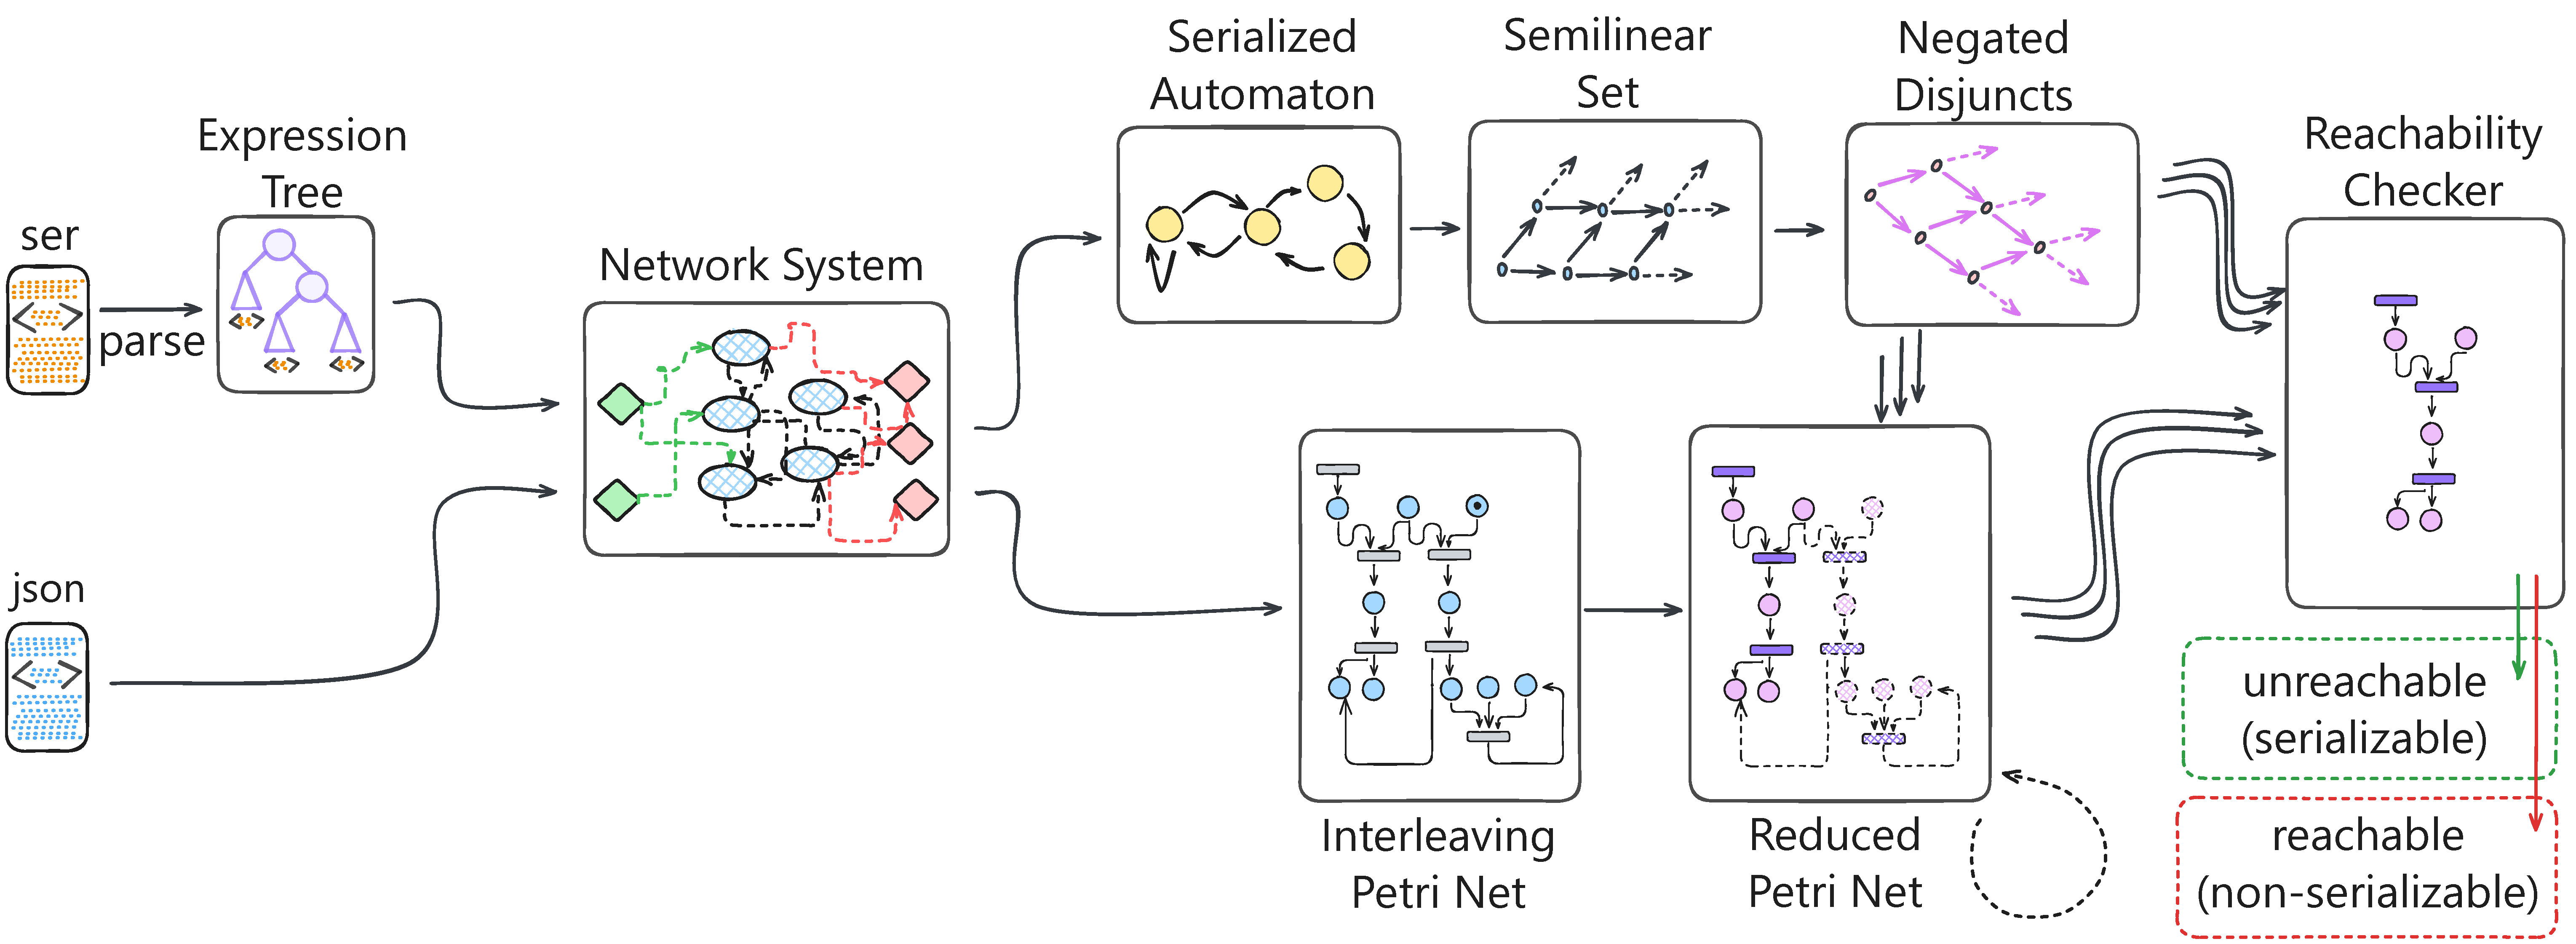
\includegraphics[width=1.0\textwidth]{plots/full_program_flow.pdf}
	\caption{Full program flow 
%		If the target set is unreachable --- a serializability proof is produced; otherwise, if it is reachable --- a counterexample trace is generated.
	(simplified, without backward arrows 
%	translating invariants (if serializable) or counterexample traces (if non-serializable) back 
	to the NS level).}
	\label{fig:full_program_flow}
\end{figure}


%\subsection{Optimizations}

%\paragraph{Bidirectional Pruning of the Petri Net}
%Before any heavy symbolic reasoning takes place, we apply bidirectional pruning on the underlying PN.  In the forward pass, we traverse from the initial marking to identify all places and transitions that could ever fire; in the backward pass, we traverse backward from any place that can influence a target constraint, and identify transitions and places that cannot contribute to reaching it.  By iteratively repeating forward passes and backward passes until convergence, we remove every component of the net that cannot both originate and contribute to the reachable target set.  This dramatically shrinks the net in practice, often converting an intractably large model into one small enough for exhaustive analysis.
%%
%We depict this in Fig.~\ref{fig:bidirectional_pruning}, and give a formal proof of correctness in Appendix~\ref{appendix:BidirectionalProof}.

%\paragraph{Redundant‐Constraint Elimination}
%When manipulating Presburger sets or their semilinear representations, it is common for some inequalities or disjuncts to add no new coverage beyond what other constraints already guarantee.  The redundant‐constraint elimination pass inspects each linear inequality and each disjunct in a disjunctive normal form, testing whether it is implied by the rest.  Any constraint or disjunct found redundant is dropped, ensuring that subsequent intersection, union, and projection operations work on the smallest necessary formula.  This streamlines the logic formula and prevents exponential blow‐up of case distinctions during solver invocations.
%
%Every time you build or star a semilinear set, you prune out any “period” vectors that are rendered useless by earlier steps:. nce you’ve accumulated a bunch of LinearSet components, you try to merge any that mathematically subsume one another:

%\paragraph{Generating Fewer Constraints}
%During set‐construction--- especially when introducing new existentially‐quantified variables or combining transition effects, we selectively avoid generating any marking that would strictly dominate an already‐seen solution.  In effect, whenever a candidate disjunct would yield a superset of an existing one, it is skipped entirely.  This ``generate‐less” heuristic stops the proliferation of large, overlapping regions in the semilinear description, trading off completeness of intermediate case‐enumeration for concise final representations.  In benchmarks with large state‐spaces, it can reduce the number of intermediate branches by orders of magnitude.

%in both the Regex and SemilinearSet Kleene-algebra instances. Concretely, instead of always building the full new structure and pruning it later, operations like union (plus) and concatenation (times) do a quick check for trivial cases and drop “zero” or “one” elements on the spo

%\paragraph{Executing Kleene Elimination in a Strategic Order:}
%When converting an NFA to a single regex, we pick the next state to eliminate by heuristically choosing the  state with the fewest incoming and outgoing edges.
%This optimization allows circumventing 
%overblown expressions resulting in naive translations, especially with regard to  Kleene closures (the “\(\mathsf{*}\)” operator).  Instead, we analyze the structure of sub-expressions under the various operators --- estimating their branching factor, and reorder them so that simpler, low‐branching components are expanded first.  This adaptive ordering often leads to early detection of fixed points or dead‐ends, preventing the combinatorial explosion that arises when complex loops are expanded prematurely.  




\subsection{Benchmark Overview} 
\label{subsec:benchmarks}
To the best of our knowledge, ours is the first and only tool to: (i) statically check serializability on \textit{unbounded} programs; and (ii) \textit{prove serializability holds}.
%
Thus, due to a lack of standard benchmarks for evaluating serializability, we 
assembled a suite of dozens of benchmarks (as part of our accompanying artifact~\cite{ArtifactRepository}).
These include both serializable and non-serializable instances encoded in both \texttt{SER} and \texttt{JSON} formats, and covering a broad range of features, including arithmetic, locks, loops, non-determinism, and more (see an overview of all our benchmarks in Table~\ref{tab:benchmarks-all} of Appendix~\ref{appendix:full_results}).
%
We note that although the benchmarks themselves are not the main part of the paper, we believe that they have merit on their own, due to their relevance to various real-world systems of interest.
%
Specifically, we wish to note our suite of benchmarks encoding \textit{network \& system protocols} (see Table~\ref{tab:networking-benchmarks}), which include stateful firewalls, BGP routing programs, network monitors, and more --- 
%highlighting the serializability challenges inherent in real-world distributed programs.
%
%Here, we were motivated by 
as motivated by real-world concurrency problems in this domain. One such example is our \textit{routing-cycle benchmark} in software-defined networks (motivated by~\cite{NaGhSa24}). Another real-world example is our \textit{snapshot isolation benchmark} (see Appendix~\ref{appendix:tour}), that was motivated by a real database bug, namely, duplicate-key errors~\cite{cockroach-issue-14099} in the popular \texttt{CockroachDB} system~\cite{cockroachdb-si-docs}.
%
In both cases and others, the non-serializable behavior was automatically identified by our toolchain.
%
%Our benchmarks include both serializable and non-serializable instances, and their features and categorization appears in Table~\ref{tab:benchmarks-all}. 



%As there are no standard benchmarks for evaluating serializability, we wrote dozens of programs in our abstract NS language. These benchmarks span a wide range of complexity --- covering branching, looping constructs, arithmetic, non-deterministic choice, and multi-request workflows that manipulate both shared (global) variables and per-request (local) state. 
%
%We include both serializable and non-serializable instances and summarize the benchmarks' features and categorizations in Table~\ref{tab:benchmarks-all}. 
%
%In particular, our most sophisticated examples are drawn from realistic networking and system-protocol scenarios, including stateful firewalls, BGP routing, network monitoring, and more --- highlighting the serializability challenges inherent in real-world distributed programs.
%
%As there are no official benchmarks for evaluating serializability, we hand-coded dozes of programs in our abstract network-system language.
%%
%The benchmarks vary in the complexity, and have multiple features: branching, loops, arithmetic, non-determinism, and multiple requests and responses, operating on both shared (global) variables and per-request (local) variables.
%%
%The benchmarks include both serializable and non-serializable instances, as we summarize in Table.~\ref{tab:benchmarks-all}, based on a category and feature-wise breakdown.
%%
%Especially, we wish to note the final category of complex examples as motivated by real-world systems and networking programs.
%%
%These include a stateful firewall, BGP routing, network monitoring and additional examples.
%
%\begin{itemize}
%		
%	\item \todo{update benchmark overview and category names}
%	\item \textbf{Core expressions \& multi request workflows}: Benchmarks testing arithmetic, boolean, and simple control expression.
%	\item \textbf{Fred (mixed arithmetic)}: Mixed control and arithmetic transformations (Fred series).
%	\item \textbf{Stop (circular-increment) series}: Circular increment loops and variants.
%	\item \textbf{Concurrency \& locking loops}: Concurrent looping patterns with locking and tricky interactions.
%	\item \textbf{Non-deterministic choice \& randomness}: Random choice and non-deterministic branching benchmarks.
%	\item \textbf{Networking \& system protocols}: Networking protocols and system-level monitoring.
%	\item \textbf{JSON state-machine examples}: Example JSON-encoded state machine workflows.
%\end{itemize}
%
%
%
%The benchmarks differ in their complexity and in the various features pertaining to them --- branching, loops, randomness, multiple requests, etc. 
%



\newpage